\documentclass[titlepage,landscape]{seminar}
\usepackage{url}
\usepackage{graphicx}
\usepackage{hyperref}
\usepackage{epstopdf}
\usepackage{slides}

\newcommand{\frack}{\frac{1}{k}}

\begin{document}

\myslide{
\heading{Where we're headed}
\[
\Var(P) = \Var(G) + \Var(E)
\]
\vfill
\[
h^2_n = \frac{\Var(A)}{\Var(P)}
\]
\vfill
\[
R = h^2_nS
\]
}

\myslide{
  \heading{Genotypic and additive genotypic values}
\begin{center}
\begin{tabular}{l|ccc}
\hline\hline
Genotype                 & $A_1A_1$    & $A_1A_2$ & $A_2A_2$ \\
\hline
Frequency                & $p^2$       & $2pq$    & $q^2$ \\
Genotypic value          & $x_{11}$    & $x_{12}$ & $x_{22}$ \\
Additive genotypic value & $2\alpha_1$ & $\alpha_1 + \alpha_2$ 
                                                  & $2\alpha_2$ \\
\hline
\end{tabular}
\end{center}
}

\myslide{
  \heading{Partitioning the genetic variance}
\begin{eqnarray*}
V_g &=&\ p^2[x_{11} - {\bar x}]^2 + 2pq[x_{12} - {\bar x}]^2
     + q^2[x_{22} - {\bar x}]^2 \label{eq:v-g} \\
    &=&\ p^2[x_{11} - 2\alpha_1 + 2\alpha_1 - {\bar x}]^2
     + 2pq[x_{12} - (\alpha_1 + \alpha_2) + (\alpha_1 + \alpha_2)
                - {\bar x}]^2 \nonumber \\
     &&\ \ + q^2[x_{22} - 2\alpha_2 + 2\alpha_2 - {\bar x}]^2
     \nonumber \\
    &=&\ p^2[x_{11} - 2\alpha_1]^2 + 2pq[x_{12} - (\alpha_1+\alpha_2)]^2
       + q^2[x_{22} - 2\alpha_2]^2 \nonumber \\
     &&\ + p^2[2\alpha_1 - {\bar x}]^2 + 2pq[(\alpha_1 + \alpha_2) - {\bar x}]^2
       + q^2[2\alpha_2 - {\bar x}]^2 \nonumber \\
     &&\ + p^2[2(x_{11} - 2\alpha_1)(2\alpha_1 - {\bar x})] \\
     &&\ +2pq[2(x_{12} - \{\alpha_1+\alpha_2\})(\{\alpha_1+\alpha_2\} -
     {\bar x})] \nonumber \\
     &&\ +q^2[2(x_{22} - 2\alpha_2)(2\alpha_2 - {\bar x})] \quad .
\end{eqnarray*}
}

\myslide{
  \heading{Covariance between half sibs}
  \vfill
TAMO
\[
\Cov(S_1, S_2) = \left({1 \over 4}\right)V_a
\]
\vfill
}

\myslide{
  \heading{Covariance among relatives}

  \begin{center}
\begin{tabular}{ll}
\hline\hline
MZ twins ($\Cov_{MZ}$) & $V_a + V_d$ \\
Parent-offspring ($\Cov_{PO}$)$^1$ & $\left(\frac{1}{2}\right)V_a$ \\
Full sibs ($\Cov_{FS}$) & $\left(\frac{1}{2}\right)V_a +
\left(\frac{1}{4}\right)V_d$ \\
Half sibs ($\Cov_{HS}$) & $\left(\frac{1}{4}\right)V_a$ \\
\hline
\multicolumn{2}{l}{$^1$One parent or mid-parent.}
\end{tabular}
\end{center}
}

\myslide{
  \heading{Evolution of quantitative traits}
  Phenotypes
\begin{eqnarray*}
F_{ij}(x) &=& \mbox{Probability that phenotype of $A_iA_j < x$} \\
x_{ij} &=& \int_{-\infty}^{\infty} x \mbox{dF}_{ij}(x) \quad
           \mbox{(genotypic value of $A_iA_j$)}
\end{eqnarray*}
\vfill
Fitness
\begin{eqnarray*}
w(x) &=& \mbox{Fitness of individual with phenotype $x$} \\
w_{ij} &=& \int_{-\infty}^{\infty}w(x) \mbox{dF}_{ij}(x)
\end{eqnarray*}
}

\myslide{
  \heading{Evolution of quantitative traits}
\begin{eqnarray*}
{\bar x}(p') &=& {\bar x}(p) + (p' - p)\left({d{\bar x} \over dp}\right)
             + o(p^2) \\
\\
{\bar x}(p) &=& p^2x_{11} + 2pqx_{12} + q^2x_{22} \\
\\
\frac{d{\bar x(p)}}{dp}
         &=& 2px_{11} + 2qx_{12} - 2px_{12} - 2qx_{22} \\
         &=& 2\left\{
             \left(px_{11} + qx_{12} - {\bar x}/2\right) +
             \left(px_{12} + qx_{22} - {\bar x}/2\right)\right\} \\
         &=& 2\left(\alpha_1 - \alpha_2\right) \\
\\
{\bar x}(p') &\approx& {\bar x}(p) + (p' - p)\left(2(\alpha_1 - \alpha_2)\right) \\
\\
\Delta{\bar x} &=& (\Delta p)\left(2(\alpha_1 - \alpha_2)\right)
\end{eqnarray*}
}

\myslide{
  \heading{Evolution of quantitative traits}
\[
p' = {p^2w_{11} + pqw_{12} \over \bar w} \quad .
\]
Thus,
\begin{eqnarray*}
   \Delta p &=& p' - p \\ 
            &=& {p^2w_{11} + pqw_{12} \over \bar w} - p \\ 
            &=& {p^2w_{11} + pqw_{12} - p\bar w \over \bar w} \\ 
            &=& p\left(pw_{11} + qw_{12} - \bar w \over \bar w \right) \quad .
\end{eqnarray*}
}

\myslide{
  \heading{Evolution of quantitative traits}

  \noindent Linear regression of fitness on phenotype:

\noindent Slope:
\[
\beta_1 = {\Cov(w,x) \over \Var(x)}
\]
Intercept
\[
\beta_0 = \bar w - \beta_1 \bar x \quad .
\]
\vfill
Fitnesses:
\begin{eqnarray*}
w_{ij} &=& \int_{-\infty}^\infty w(x) \mbox{\rm dF}_{ij}(x) \\
       &\approx& \int_{-\infty}^\infty (\beta_0 + \beta_1x) \mbox{\rm dF}_{ij}(x) \\
       &=& \beta_0 + \beta_1x_{ij} \\
\bar w &\approx& \beta_0 + \beta_1\bar x \quad .
\end{eqnarray*}
}

\myslide{ 
  \heading{Evolution of quantitative traits}

  \begin{eqnarray*}
   \Delta p &=& p\left(pw_{11} + qw_{12} - \bar w \over \bar w \right) \\
            &\approx& p\left(p(\beta_0 + \beta_1x_{11}) 
                      + q(\beta_0 + \beta_1x_{12})
                      - (\beta_0 + \beta_1\bar x) \over \bar w \right) \\
            &=& p\beta_1\left(px_{11} + qx_{12} - \bar x \over 
                             \bar w \right) \\
            &=& p\beta_1\left(\alpha_1 - \bar x/2 \over \bar w \right) \\
            &=& p\beta_1\left(\alpha_1 - (p\alpha_1 + q\alpha_2) \over
                             \bar w \right) \\
            &=& {pq\beta_1(\alpha_1 - \alpha_2) \over \bar w} \quad .
\end{eqnarray*}
}

\myslide{
  \heading{Evolution of quantitative traits}

  \begin{eqnarray*}
\Delta{\bar x} &=& (\Delta p)\left(2(\alpha_1 - \alpha_2)\right) \\
&=& \left(\frac{pq\beta_1(\alpha_1 - \alpha_2)}{\bar w}\right)
\left(2(\alpha_1 - \alpha_2)\right) \\
&=& \frac{2pq\beta_1(\alpha_1 - \alpha_2)^2}{\bar w} \\
&=& \frac{V_a\beta_1}{\bar w}
\end{eqnarray*}
}

\myslide{
  \heading{Evolution of quantitative traits}

  \begin{eqnarray*}
\Cov(w,x) &=& p^2\int_{-\infty}^\infty x w(x) \mbox{\rm dF}_{11}(x)
            + 2pq\int_{-\infty}^\infty x w(x) \mbox{\rm dF}_{12}(x) \\
         && \qquad + q^2\int_{-\infty}^\infty x w(x) \mbox{\rm dF}_{22}(x)
            - \bar x \bar w \\
         &=& p^2\left(\int_{-\infty}^\infty x w(x) \mbox{dF}_{11}(x) - 
            x_{11}\bar w\right) \\
         && \quad + 2pq\left(\int_{-\infty}^\infty x w(x)
            \mbox{dF}_{11}(x) -
            x_{12}\bar w\right) \\
         && \quad + q^2\left(\int_{-\infty}^\infty x w(x) \mbox{dF}_{22}(x) - 
            x_{22}\bar w\right) \quad .
\end{eqnarray*}
}

\myslide{
  \heading{Evolution of quantitative traits}

  \begin{eqnarray*}
\int_{-\infty}^\infty x w(x) \mbox{\rm dF}_{ij}(x) - x_{ij}\bar w 
              &=& \bar w \left(
                 \int_{-\infty}^\infty {x w(x) \over \bar w} \mbox{\rm
                 dF}_{ij}(x)
                 - x_{ij}
                 \right) \\
              &=& \bar w (x_{ij}^* - x_{ij})
\end{eqnarray*}
\vfill
\begin{eqnarray*}
\Cov(w,x) &=& p^2\bar w(x_{11}^* - x_{11}) + 2pq\bar w(x_{12}^* - x_{12})
              q^2\bar w(x_{22}^* - x_{22}) \\
&=& \bar w(\bar x^* - \bar x)
\end{eqnarray*}
\vfill
\begin{eqnarray*}
\Delta\bar x &=& V_a \left({\bar w(\bar x^* - \bar x) \over
                               V_p} \over \bar w \right) \cr 
             &=& h^2_N (\bar x^* - \bar x) \cr
\end{eqnarray*}
}

\myslide{
  \heading{Evolution of quantitative traits}

  \begin{center}
\begin{tabular}{l|ccc}
\hline\hline
Genotype  & $A_1A_1$ & $A_1A_2$ & $A_2A_2$ \\
Phenotype & 1.303  & 1.249  & 0.948 \\
\hline
\end{tabular}
\end{center}

\noindent Assume $p=0.25$, $V_p=0.16$. This implies ${\bar x}=1.08$
and $h^2_N=0.1342$. Assume $\bar x^* = 1.544$.

\begin{eqnarray*}
S &=& \bar x^* - \bar x \\
  &=& 1.544 - 1.08 \\
  &=& 0.464 \\
\Delta\bar x &=& h^2_N S \\
         &=& (0.1342)(0.464) \\
         &=& 0.06 \\
\bar x' &=& \bar x + \Delta\bar x \\
        &=& 1.08 + 0.06 \\
        &=& 1.14 
\end{eqnarray*}
}

\myslide{
\heading{Fisher's Fundamental Theorem of Natural Selection}
  
\begin{center}
\begin{tabular}{l|ccc}
\hline\hline
Genotype                 & $A_1A_1$ & $A_1A_2$ & $A_2A_2$ \\
\hline
Frequency                & $p^2$    & $2pq$    & $q^2$ \\
Fitness                  & $w_{11}$ & $w_{12}$ & $w_{22}$ \\
Additive fitness value   & $2\alpha_1$ & $\alpha_1 + \alpha_2$ &
$2\alpha_2$ \\
\hline
\end{tabular}
\end{center}
\[
\Delta p = \left({{pq} \over 2{\bar w}}\right)
           \left({{d{\bar w}} \over {dp}}\right) \quad .
\]
\[
{\bar w}' = {\bar w} + \left(\Delta p\right)\left({{d{\bar w}} \over {dp}}\right)
            + \left({{(\Delta p)^2} \over 2}\right)
              \left({{d^2{\bar w}} \over {dp^2}}\right) \quad .
\]
Or, equivalently
\[
\Delta {\bar w} = \left(\Delta p\right)\left({{d{\bar w}} \over {dp}}\right)
            + \left({{(\Delta p)^2} \over 2}\right)
              \left({{d^2{\bar w}} \over {dp^2}}\right) \quad .
\]
}

\myslide{
\heading{Fisher's Fundamental Theorem of Natural Selection}

\begin{eqnarray*}
\frac{d{\bar w}}{dp}
 &=& 2pw_{11} + 2(1-p)w_{12} - 2pw_{12} - 2(1-p)w_{22} \\
 &=& 2[(pw_{11}+qw_{12}) - (pw_{12}+qw_{22})] \\
 &=& 2[(pw_{11}+qw_{12}-{\bar w}/2) - (pw_{12}+qw_{22}-{\bar w}/2)] \\
 &=& 2[\alpha_1 - \alpha_2] \\
 &=& 2\alpha
\end{eqnarray*}
\vfill
\begin{eqnarray*}
\frac{d^2{\bar w}}{dp^2}
 &=& 2w_{11} - 2w_{12} - 2w_{12} + 2w_{22} \\
 &=& 2(w_{11} - 2w_{12} + w_{22}) \\
\end{eqnarray*}
\vfill
\begin{eqnarray*}
\Delta {\bar w}
 &=& \left\{\left({{pq} \over {2{\bar w}}}\right)\left({{d{\bar w}} \over {dp}}\right)
      \right\}
    \left({{d{\bar w}} \over {dp}}\right)
    + {{ \left\{\left({{pq} \over {2{\bar w}}}\right)\left({{d{\bar w}} \over {dp}}\right)
      \right\}^2} \over 2}
    [2(w_{11} - 2w_{12} + w_{22})] \\
 &=& \left\{\left({{pq} \over {2{\bar w}}}\right)\left(2\alpha\right)\right\}\left(2\alpha\right)
    + \left\{\left({{pq} \over {2{\bar w}}}\right)\left(2\alpha\right)\right\}^2
    (w_{11} - 2w_{12} + w_{22}) \\
 &=& {{2pq\alpha^2} \over {\bar w}}
    + {{p^2q^2\alpha^2} \over {{\bar w}^2}}(w_{11} - 2w_{12} + w_{22}) \\
 &=& {V_a \over {\bar w}}
    \left\{1 + {{pq} \over {2{\bar w}}}(w_{11} - 2w_{12} + w_{22})\right\} \\
 &\approx& {V_a \over {\bar w}}
\end{eqnarray*}
}

\myslide{
\heading{Selection on multiple traits}

\noindent Selective differential:
\[
{\bf s} = \bar{\bf z}^* - \bar{\bf z}
\]
\vfill
\noindent $W({\bf z})$ is absolute fitness of individual
with phenotype $\bf z$
\[
\bar W = \int W({\bf z})p({\bf z})d{\bf z} \quad .
\]
\noindent Relative fitness (mean relative fitness $=$ 1)
\[
w({\bf z}) = {W({\bf z}) \over \bar W} \quad .
\]
\vfill
\[
\bar{\bf z}^* = \int {\bf z}w({\bf z})p({\bf z})d{\bf z} \quad .
\]
}

\myslide{
\heading{Selection on multiple traits}

\begin{eqnarray*}
{\bf s} &=& \bar{\bf z}^* - \bar{\bf z} \\
        &=& \int {\bf z}w({\bf z})p({\bf z})d{\bf z} - \bar {\bf z} \\
        &=& E(w,z) - \bar w\bar {\bf z} \\
        &=& \Cov(w,z)
\end{eqnarray*}
}

\myslide{
\heading{Selection on multiple traits}

\[
{\bf P} = {\bf G} + {\bf E} \quad .
\]
\vfill
\begin{eqnarray*}
\bar{\bf x}^* - \bar{\bf x} &=& {\bf GP}^{-1}(\bar{\bf z}^* - \bar{\bf z}) \\
\bar{\bf z}'  - \bar{\bf z} &=& {\bf GP}^{-1}(\bar{\bf z}^* - \bar{\bf z}) \\
\Delta\bar{\bf z} &=& {\bf GP}^{-1}{\bf s}
\end{eqnarray*}
\vfill
\[
{\bf \beta} = {\bf P}^{-1}{\bf s}
\]
\begin{eqnarray*}
s_i &=& \sum_{j=1}^n \beta_jP_{ij} \\
    &=& \beta_1P_{i1} + \cdots + \beta_iP_{ii} + \cdots + \beta_nP_{in}
\end{eqnarray*}
}

\myslide{
\heading{Selection on multiple traits}

\begin{center}
\begin{tabular}{l|cc}
\hline\hline
Character & Mean before selection & standard deviation \\
\hline
head      & 0.880                 & 0.034 \\
thorax    & 2.038                 & 0.049 \\
scutellum & 1.526                 & 0.057 \\
wing      & 2.337                 & 0.043 \\
\hline
\end{tabular}
\vskip 4pt
\begin{tabular}{l|cccc}
\hline\hline
          & head & thorax & scutellum & wing \\
\hline
head      & 1.00 & 0.72   & 0.50      & 0.60 \\
thorax    &      & 1.00   & 0.59      & 0.71 \\
scutellum &      &        & 1.00      & 0.62 \\
wing      &      &        &           & 1.00 \\
\hline
\end{tabular}
\end{center}
}

\myslide{
\heading{Selection on multiple traits}

\begin{center}
\begin{tabular}{l|cccc}
\hline\hline
Character & $s$    & $s'$  & $\beta$ & $\beta'$ \\
\hline
head      & -0.004 & -0.11 & -0.7 $\pm$ 4.9 & -0.03 $\pm$ 0.17 \\
thorax    & -0.003 & -0.06 & 11.6 $\pm$ 3.9$^{**}$ & 0.58 $\pm$ 0.19$^{**}$
\\
scutellum & -0.16$^*$ & -0.28$^*$ & -2.8 $\pm$ 2.7 & -0.17 $\pm$ 0.15 \\
wing      & -0.019$^{**}$ & -0.43$^{**}$ & -16.6 $\pm$ 4.0$^{**}$ & -0.74 $\pm$
0.18$^{**}$ \\
\hline
\end{tabular}
\end{center}
}

\myslide{
  \heading{Association mapping}

  \noindent Na\"ive approach. Regression of phenotype on genotype:
  \[
    y_i = x_{ij}\beta_j + \epsilon_{ij} \quad ,
  \]
  where $y_i$ is the phenotype of individual $i$, $x_{ij}$ is the
  genotype of individual $i$ at locus $j$ (0, 1, 2), and
  $\epsilon_{ij} \sim \mbox{N}(0, \sigma^2)$ is the error.
  \vfill
  {\color{red}\bf PROBLEM}: Individuals may be similar to one another
  because of genetic similarity not reflected in the particular
  markers chosen, e.g., relatedness within a population, population
  structure
}

\myslide{
  \heading{Association mapping}

  \noindent Better approach. Regression of phenotype on genotype with
  a random effect reflecting genetic similarity at markers not
  included in the analysis

  \[
    y_i^{(k)} = x_{ij}\beta_j + \phi^{(k)} + \epsilon_{ij}
  \]

  In general $\phi^{(k)}$ may reflect a general measure of
  relatedness, usually estimated from SNPs.
}

\myslide{
\heading{Warfarin resistance}
\vfill
\begin{center}
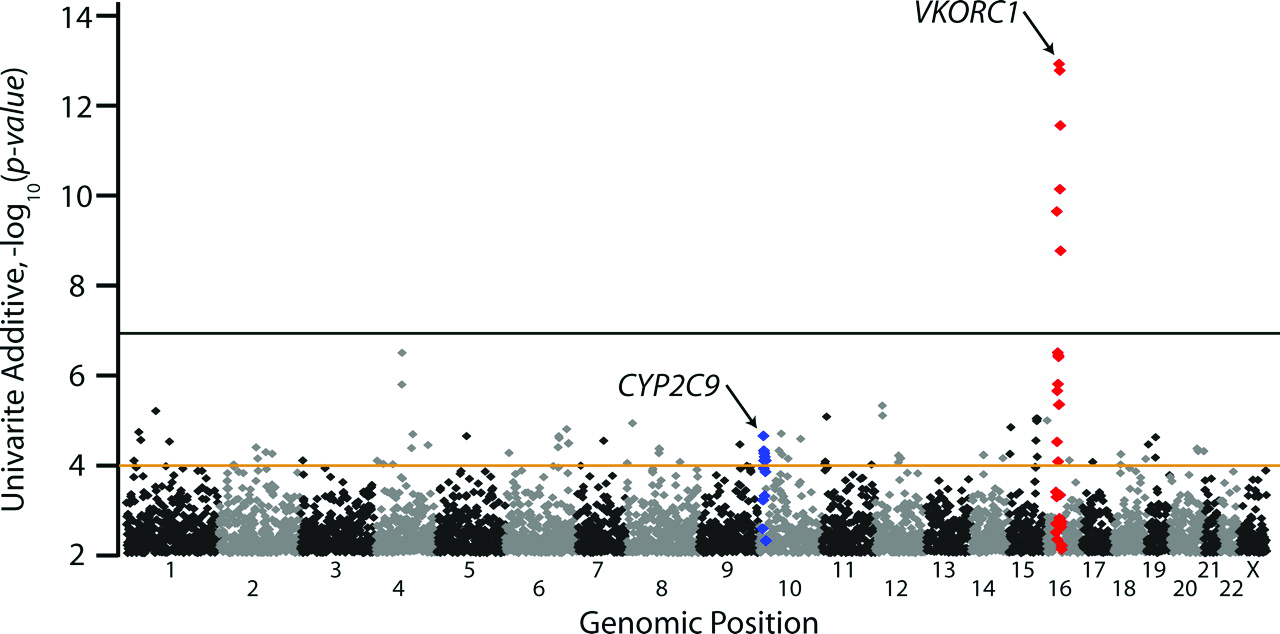
\includegraphics[width=0.9\textwidth]{GWAS-warfarin.eps}
\end{center}
}

\myslide{
  \heading{Two-locus population genetics}
\begin{center}
\begin{tabular}{lcccc}
Gamete    & $A_1B_1$ & $A_1B_2$ & $A_2B_1$ & $A_2B_2$ \\
Frequency & $x_{11}$ & $x_{12}$ & $x_{21}$ & $x_{22}$
\end{tabular}
\end{center}
\vfill
If alleles are arranged randomly into gametes then,
\begin{eqnarray*}
x_{11} &=& p_1p_2 \\
x_{12} &=& p_1q_2 \\
x_{21} &=& q_1p_2 \\
x_{22} &=& q_1q_2 \quad ,
\end{eqnarray*}
where $p_1 = \hbox{freq}(A_1)$ and $p_2 = \hbox{freq}(A_2)$.
}

\myslide{
  \heading{Two-locus population genetics}

  In general,
  \begin{eqnarray*}
    x_{11} &=& p_1p_2 + D \\
    x_{12} &=& p_1q_2 - D \\
    x_{21} &=& q_1p_2 - D \\
    x_{22} &=& q_1q_2 + D \\
    \\
    D &=& x_{11}x_{22} - x_{12}x_{21}
  \end{eqnarray*}

  \vfil
  
  $D$: gametic disequilibrium

  \vfill
}

\myslide{
  \heading{Two-locus population genetics}
\[
\begin{array}{ccccccc}
    &\mu_1            &     &      &     &\mu_2 \\
A_1 &\rightleftharpoons& A_2 &\qquad& B_1 &\rightleftharpoons& B_2
\quad , \\
    &\nu_1            &     &      &     &\nu_2 
\end{array}
\]
\vfill
\begin{eqnarray*}
\frac{\mbox{E}(D^2)}{\mbox{E}(p_1(1-p_1)p_2(1-p_2))}
&\approx& \frac{1}{3 + 4N_er}
\end{eqnarray*}
}

\myslide{
  \heading{Two-locus population genetics}
\begin{center}
\begin{tabular}{c|cccc|cc|c}
\hline\hline
           & \multicolumn{4}{c|}{Gamete frequencies} 
           & \multicolumn{2}{c|}{Allele frequencies} \\
Population & $A_1B_1$ & $A_1B_2$ & $A_2B_1$ & $A_2B_2$ 
           & $p_{i1}$ & $p_{i2}$ & $D$ \\
\hline
1          & 0.24     & 0.36     & 0.16    & 0.24
           & 0.60     & 0.40     & 0.00 \\
2          & 0.14     & 0.56     & 0.06    & 0.24
           & 0.70     & 0.20     & 0.00 \\
Combined   & 0.19     & 0.46     & 0.11    & 0.24
           & 0.65     & 0.30     & -0.005 \\
\hline
\end{tabular}
\end{center}
}

\myslide{
  \heading{Two-locus population genetics}
\begin{eqnarray*}
D_i &=& x_{11,i} - p_{1i}p_{2i} \\
D_t &=& \bar x_{11} - \bar p_1\bar p_2 \\
\bar x_{11} &=& \frac{1}{K} \sum_{k=1}^K x_{11,k} \\
\bar p_1 &=& \frac{1}{K} \sum_{k=1}^K p_{1k} \\
\bar p_2 &=& \frac{1}{K}\sum_{k=1}^K p_{2k}
\end{eqnarray*}
}

\myslide{
  \heading{Two-locus population genetics}
\begin{eqnarray*}
D_t &=& \bar x_{11} - \bar p_1\bar p_2 \\
    &=& \frac{1}{K} \sum_{k=1}^K x_{11,k} - \bar p_1\bar p_2 \\
    &=& \frac{1}{K} \sum_{k=1}^K (p_{1k}p_{2k} + D_k) - \bar p_1\bar p_2 \\
    &=& \frac{1}{K} \sum_{k=1}^K (p_{1k}p_{2k} - \bar p_1\bar p_2) + \bar D \\
    &=& \mbox{Cov}(p_1, p_2) + \bar D \quad ,
\end{eqnarray*}
}

\myslide{
  \heading{Two-locus population genetics}
\begin{eqnarray*}
\mbox{Cov}(p_1, p_2) &=& 0.5(0.6-0.65)(0.4-0.3) + 0.5(0.7-0.65)(0.2-0.3) \\
                     &=& -0.005 \\
\bar x_{11}          &=& (0.65)(0.30) - 0.005 \\
                     &=& 0.19 \\
\bar x_{12}          &=& (0.65)(0.7) + 0.005 \\
                     &=& 0.46 \\
\bar x_{21}          &=& (0.35)(0.30) + 0.005 \\
                     &=& 0.11 \\
\bar x_{22}          &=& (0.35)(0.70) - 0.005 \\
                     &=& 0.24 \quad .
\end{eqnarray*}
}

\end{document}
